% -*- root: main.tex -*-
%-------------------------------------------------------------------------------
\chapterimage{chapter_head_1.pdf} 

%-------------------------------------------------------------------------------
\chapter{로봇 운영 체제}

%-------------------------------------------------------------------------------
\section{로봇 소프트웨어 플랫폼}\index{로봇 소프트웨어 플랫폼}

%-------------------------------------------------------------------------------
\subsection{플랫폼이 가져온 변화}\index{플랫폼이 가져온 변화}

잠깐, 로봇 이야기가 아닌, 핸드폰에 대해서 이야기해보자. 불가 20년전만 하더라도 스마트폰과 같은 핸드폰이 지금과 같이 많은 사람들의 필수품이 되리라고는 생각지도 못했었다.
더욱이, 초기의 핸드폰은 핸드폰이라는 이름이 무상할 정도로 크고 무거운 무전기와 같았고, 가격은 상상을 초월할 정도로 비쌌으며, 성능은 떨어졌다.
이에 비하여 현재의 스마트폰은 가격도 저렴하고, 가볍고, 작고 사용하기도 편리하다는 것을 본다면 그 변화는 놀랍기까지 하다.

\begin{figure}[h]
\centering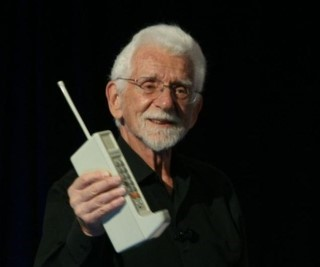
\includegraphics[width=0.5\columnwidth]{pictures/chapter1/motorola_dynatac.jpg}
\caption{올해로 40주년이 된 최초 상용 핸드폰 모토롤라 다이나택 8000 와 개발자 Martin Cooper}
\end{figure}

올해 2013년, 40주년이 된 세계 최초의 상용 핸드폰인 모토롤라 다이나택 8000의 경우\footnote{http://www.segye.com/content/html/2013/04/04/20130404004829.html}\footnote{CarToyBlog, "Happy 40th Birthday to the Cell Phone!",  http://blog.cartoys.com/date/2013/04/},\footnote{http://venma.tistory.com/entry/Motorola-DynaTAC-8000X}, 그 당시 가격으로 500만원대, 0.8Kg의 무게, 최대 통화시간 30분, 충전 10시간 소요, 최대 30개 전화번호 입력 정도만이 가능하였다.
그 뒤로 핸드폰 시장은 급성장하게 되었고, 현재의 스마트폰까지 이르렀다. 그리고, 지금은 우리에게는 없어서는 안되는 생활 필수 아이템이 되었다.

그렇다면 이러한 것이 가능했던 이유는 무엇이였을까? 

초기에 많은 핸드폰 관련 회사들은 기술 경쟁을 거듭하며, 슬림하면서도 가볍고 고화질, 고음질, 휴대성 등 자신들만의 특징들을 네세우며 새로운 기기들을 내놓았다.
그 당시만해도 핸드폰은 모델마다 하드웨어에 맞게 기능을 추가하기 위하여 하드웨어 의존적인 펌웨어 개발을 했다.
한 회사에만 수 십가지 기종이 있었을테고, 전세계적으로는 어땠을까?
상상할 수도 없는 규모이다.
목적은 다 비슷한데 통합되지 못하고 그렇게 개발자들은 죽어라~ 새로운 하드웨어 개발 일정에 맞추어 펌웨어 개발을 했고 이는 반복되었다.
새로운 하드웨어마다 의존적으로 개발하였기에 그 발전 속도는 떨어졌고, 의존성으로 인하여 관리 비용은 높기만 했다.
그리고 그 비용은 우리 소비자의 몫이였다. 

\begin{figure}[h]
\centering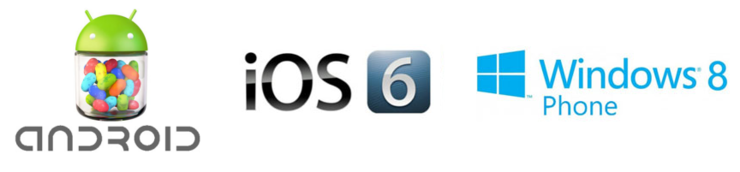
\includegraphics[width=\columnwidth]{pictures/chapter1/oss.png}
\caption{다양한 OS}
\end{figure}

지금은 어떠한가? 안드로이드, iOS, 윈도우즈 등 대표적인 OS를 기반으로 개발자들이 힘을 모으게 되었고 이러한 소프트웨어 플랫폼을 기반으로 핸드폰이라는 하드웨어 플랫폼을 잘 몰라도 관련 어플리케이션 개발에 문제가 없게 되었다.
그리고, 앱 개발자라는 새로운 소프트웨어 직종을 생길 정도로 스마트폰 운영체제를 기반으로 한 개발 환경이 확립되었으며, 스마트폰 운영체제 관리팀 이외에도 스마트폰 회사, 앱 개발자, 심지어 일반 사용자들까지도 하나로 뭉쳐서 하드웨어와 소프트웨어를 통합하는 플랫폼은 진화의 진화를 거듭하게 되었다.
이는 핸드폰 뿐만아니라 개인컴퓨터 개발과 더불어 불어닥친 유닉스, 리눅스, 윈도우, OS X 등의 컴퓨터용 OS 도 마찬가지 양상이라고 볼 수 있다.

이러한 이유로는 하드웨어의 급성장과 필연적인 사용자들의 수요도 있었겠지만,  소프트웨어 플랫폼 기반으로 지식이 한데 모아져서 나온 결과라고 볼 수 있다.
이러한 소프트웨어 플랫폼은 하드웨어 플랫폼의 인터페이스를 통합시키게 만들고, 나아가 하드웨어를 몰라도 상위 단의 프로그램인 응용 프로그램에 집중할 수 있게 되었기 때문에 사용자들의 수요에 맞는 응용 제품이 나올 수 있었다고 생각된다. 

%-------------------------------------------------------------------------------
\subsection{플랫폼이 가져온 변화}\index{플랫폼이 가져온 변화}

최근, 로봇계도 마찬가지의 움직임을 보이고 있다. 스마트폰 OS 나 개인컴퓨터 OS 에 비하여 그 규모는 작고, 아직 발전 단계이기는 하지만 로봇 소프트웨어 플랫폼은 춘추전국시대라고 볼 수 있을 정도로 매우 활발하게 진행되고 있다.
아래의 리스트는 그 중에서 돋보이는 활동을 보이고 있는 그룹들의 로봇 소프트웨어 플랫폼이다.

\begin{itemize}
\item ERSP,Evolution robotics (회사)\footnote{http://www.evolution.com/products/ersp/}
\item MSRDS,Microsoft (회사)\footnote{http://msdn.microsoft.com/en-us/robotics/default.aspx}
\item OpenRTM,일본의 AIST (국립 연구소)\footnote{http://www.openrtm.org}
\item ROS,Open Source Robotics Foundation\footnote{http://www.osrfoundation.org/}
\item OROCOS,유럽\footnote{http://www.orocos.org/}
\item OPRoS,한국\footnote{http://www.opros.or.kr/}
\end{itemize}

\begin{figure}[h]
\centering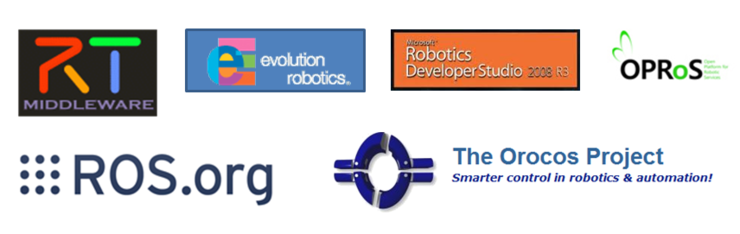
\includegraphics[width=\columnwidth]{pictures/chapter1/robotplatforms.png}
\caption{다양한 로봇 소프트웨어 플랫폼}
\end{figure}

위와 같이 많은 플랫폼들이 등장하고 있고, 현재도 다양한 접근방식으로 증가 추세에 있다.
너도나도 로봇계의 로봇 소프트웨에 플랫폼의 선두에 서고 싶기 때문일 것이다.
현재, 다양한 로봇 소프트웨어 플랫폼이 나오고 있지만, 어느 것이 좋다라고는 섣불리 말하기 어려운게 사실이다.
그러나, 언젠가는 지금의 운영체제들처럼 독특한 스타일은 있을지는 몰라도 사용자 측면에서는 궁극적으로 비슷한 기능들로 압축 될 것이라고 생각한다.
우리는 소프트웨어 플랫폼 자체를 만드는 것이 아닌, 범용적인 로봇 소프트웨어 플랫폼에서도 돌아갈 수 있는 응용 프로그램 개발 능력에 집중하면 좋을 듯 싶다.
예를들어 안드로이드 어플 개발과 iOS 어플 개발이 비슷해진 것을 예를 들 수 있다. 

그렇다면 우리는 현재 나와있는 로봇 소프트웨어 플랫폼 중에서 어떤것을 우선적으로 익혀두면 좋을까?
필자는 이 중 어떤 것이 나에게 제일 적합하고, 앞으로 장래성이 있을까?
그리고 커뮤니케이션은?
오픈소스인가?
개발 환경은 어떻게 지원될까?
이러한 질문에서 가장 정답으로 생각하는 것은 Open Source Robotics Foundation 의 ROS라고 생각한다.
특히, 커뮤니티의 활발성, 준비되어 있는 라이브러리, 확장성, 개발 편의성을 생각해본다면 ROS 만한 것도 없어 보인다.
이 춘추전국시대와 같은 다양한 로봇 소프트웨어 플랫폼 중에서 어떤것이 살아 남을지 필자도 매우 궁금하다.

%-------------------------------------------------------------------------------
\subsection{로봇 소프트웨어 플랫폼이 가져올 미래}\index{로봇 소프트웨어 플랫폼이 가져올 미래}

로봇 소프트웨어 플랫폼은 정해진 하드웨어 플랫폼을 기준으로 하고 있기에 소프트웨어 플랫폼을 이용하면 하드웨어에 대한 지식이 없어도 응용 프로그램을 작성 가능하다.
이는 최신 스마트폰의 하드웨어 구성 및 세부 내역을 몰라도 어플을 작성가능한 것과 마찬가지이다.
또한, 로봇 개발자가 하드웨어 설계부터 소프트웨어 설계까지 하던 이전 작업 프로세서와 구별되어 더 많은 소프트웨어 인력들이 로봇 응용 제품에 참여 할 수 있다.
즉, 소프트웨어 플랫폼의 역할로 많은 이들이 로봇 개발에 동참하게 되는 길을 열고, 하드웨어는 소프트웨어 플랫폼을 사용하기 위하여 소프트웨어 플랫폼에서 제안하는 인터페이스에 맞도록 설계가 될것이다.
이는 로봇 개발이 급속도로 발전 할 수 있는 계기를 마련하게 되는 것이라고 생각한다.

%-------------------------------------------------------------------------------
\section{ROS 소개}\index{ROS 소개}

%-------------------------------------------------------------------------------
\subsection{ROS 란?}\index{ROS 란?}

ROS is an open-source, meta-operating system for your robot.
It provides the services you would expect from an operating system, including hardware abstraction, low-level device control, implementation of commonly-used functionality, message-passing between processes, and package management.
It also provides tools and libraries for obtaining, building, writing, and running code across multiple computers\footnote{http://wiki.ros.org/ROS/Introduction}.

\begin{figure}[h]
\centering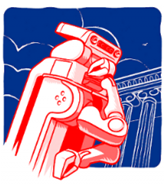
\includegraphics[width=0.2\columnwidth]{pictures/chapter1/think_pr2.png}
\caption{생각하는 PR2 (http://www.willowgarage.com/blog)}
\end{figure}

ROS 위키에는 위와 같은 정의를 내리고 있다. ROS는 로봇 응용프로그램을 개발할때 필요한 하드웨어 추상화, 하위 디바이스 제어, 일반적으로 사용되는 기능의 구현, 프로세스간의 메시지 패싱, 패키지 관리, 개발환경에 필요한 라이브러리와 다양한 개발 및 디버깅 도구를 제공한다는 것이다. 

즉, ROS는 로봇 응용 프로그램을 개발을 위한 운영체제와 같은 로봇 플랫폼이다.
이는 하드웨어 플랫폼을 하드웨어 추상화로 포함하고 있으며, 로봇 응용 소프트웨어 개발을 지원을 위한 소프웨어 플랫폼이면서 이기종의 하드웨어에서 사용 가능한 운영 체제와 같은 기능을 갖추고 있다.

%-------------------------------------------------------------------------------
\subsection{ROS는 새로운 운영체제(OS)인가?}\index{ROS는 새로운 운영체제(OS)인가?}

범용 컴퓨터의 경우, Windows(Windows XP, 7, 8 ...), Linux(Ubuntu, Fedora, Gentoo ...), MAC(OS X ...)가 있으며, 스마트폰의 경우에는 Android, iOS, Symbian, RiMO, Bada 등 많은 OS가 있다.
모두 전통적인 OS(Operating System)에 속하게 된다.
정말 다양한 하드웨어에 수 많은 OS의 종류가 있다. 

ROS는 Robot Operating System 이라고 하여 OS 임을 나태내고 있다.
특히, ROS를 처음 접한 사람들은 ROS를 전통적인 운영체제라고 생각하는 경우가 있다.
필자 역시, 처음에는 ROS가 로봇을 위한 새로운 운영체제라고 생각하였다. 

그러나, No!, ROS은 메타운영체제(Meta-Operating System)이다.

메타운영체제(Meta-Operating System) 딱히 정확히 정의된 용어는 아니지만, 어플리케이션과 분산 컴퓨팅 자원간의 가상화 레이어로 분산 컴퓨팅 자원을 활용하여, 스케쥴링 및 로드, 감시, 에러 처리 등을 실행하는 시스템이라고 볼 수 있다.
즉, 윈도우, 리눅스, 안드로이드와 같은 전통적인 운영체제는 아니다.
오히려, ROS는 기존의 전통적인 운영체제(리눅스,윈도우,OS-X,안드로이드)를 이용하고 있다.
리눅스의 한 배포판인 Ubuntu과 같은 운영체제의 프로세스 관리 시스템, 파일 시스템, 유저 인터페이스, 프로그램 유틸(컴파일러, 스레드 모델 등)등을 사용하고 있다.
이에 추가적으로 다수의 이기종 하드웨어간의 데이터 송수신, 스케쥴링, 에러 처리 등 로봇 응용 소프트웨어에 필요한 필수 기능들을 라이브러리 형태로 제공하고 있다.
또한, 이러한 기반 로봇 프레임워크를 기반으로 다양한 목적의 응용 패키지를 개발, 관리, 제공하고 있으며 유저들이 개발한 패키지 또한 유통하는 생태계(ecosystem)를 갖추고 있다.

그림으로 나타내면 아래와 같다고 볼 수 있다. 기존의 전통적인 운영체제를 이용하면서, 로봇 응용 개발에 필수적인 로봇 및 센서의 하드웨어 추상화 개념으로 이를 제어하고, 유저의 로봇 응용 프로그램 개발을 위한 지원 시스템인것이다.

\begin{figure}[h]
\centering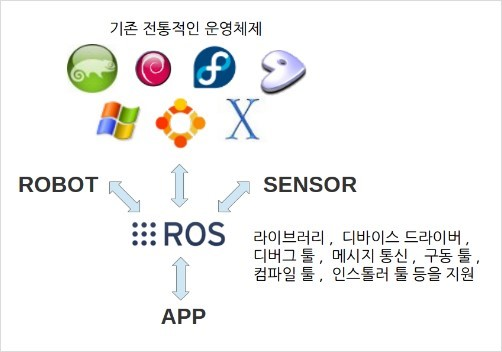
\includegraphics[width=0.7\columnwidth]{pictures/chapter1/ros_is_not_os.jpg}
\caption{메타 운양 체제로서의 ROS}
\end{figure}

또한, 아래의 그림처럼 ROS는 하나의 운영체제에서의 메시지도 지원하지만 서로 다른 운영체제, 하드웨어, 프로그램에서도 메시지 처리를 할 수가 있어서 다양한 하드웨어가 이용되는 로봇 개발에는 매우 적합한 운영체제라고 할 수 있다.
이에 대한 내용은 이어지는 강좌들에서 좀 더 자세히 다루기로 하겠다.  

\begin{figure}[h]
\centering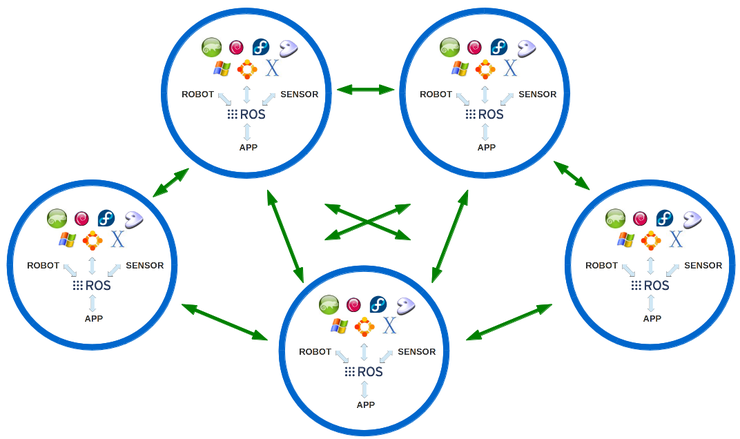
\includegraphics[width=0.9\columnwidth]{pictures/chapter1/rosmulti.png}
\caption{ROS 멀티 그룹}
\end{figure}

%-------------------------------------------------------------------------------
\subsection{ROS 생태계}\index{ROS 생태계}

스마트폰 시장에서 Android, iOS,  Symbian, RiMO, Bada 등 다양한 OS가 등장하면서 생태계(ecosystem)라는 말을 자주 듣곤 한다.
이는 스마트폰을 생산하는 하드웨어 회사와 이를 사용하는 유저 혹은 어플리케이션 소프트웨어(앱,APP) 개발자를 연결해주는 구조를 말한다.
스마트폰 회사들이 기기를 생산, 운영체제의 인터페이스에 맞추고, 각 OS 회사들은 이를 라이브러리화시켜 제공해주고, 소프트웨어 개발자들이 이를 이용하여 하드웨어 지식이 없어도 손쉽게 개발작업을 해줄 수 있는 구조, 그리고 유저가 사용하기 쉽도록 유통하는 것이 바로 생태계이다. 

이러한 생태계는 모바일 시장에서 제일 먼저 했던것은 아니다.
범용 컴퓨터 분야도 다양한 하드웨어 회사들이 있고, 이를 묶어준 것은 마이크로소프트사의 Windows OS 및 자유진영의 리눅스가 대표적이였다.
어쩜 이러한 흐름은 자연의 생태계처럼 비슷한 흐림이 아닐까 싶다. 

로봇 분야도 마찬가지 흐름으로 가고 있다.
처음에는 여러 시도로 각종 하드웨어 기술들이 넘쳐흘렀으나, 이를 통합해줄 OS가 전무했다.
이 상황에서 다양한 소프트웨어 플랫폼이 등장했고, 가장 주목받은 ROS의 경우 이제 그 생태계의 틀을 갖추기 시작했다.
아직, 그 여파력은 미미하지만 점점 늘고 있고 있는 유저들과 회사들 그리고 급격히 늘고 있는 관련 툴 및 라이브러리를 볼 때 멀지 않아 생태계가 완만히 돌아갈 것이라고 기대해본다.
그리고, 로봇회사 및 센서회사와 같은 로봇 관련 하드웨어 분야의 개발자, ROS 개발 운용 팀, 응용 소프트웨어 개발자, 유저 모두가 웃을 수 있는 생태계가 되길 바란다.
 
아래는 2013년 9월 기점으로 필자가 조사해본 ROS 실태이다\footnote{http://www.ros.org/browse/list.php}\footnote{http://www.ros.org/news/2012/12/ros-five-years.html}.
아직, 미미한 수준이라고 생각하는 사람들도 있지만, 로봇 분야에서 이만큼 세력을 키운 로봇 소프트웨어 플랫폼은 없다고 생각한다.
앞으로 어떻게 변할지 점점 기대가 된다!

\begin{figure}[h]
\centering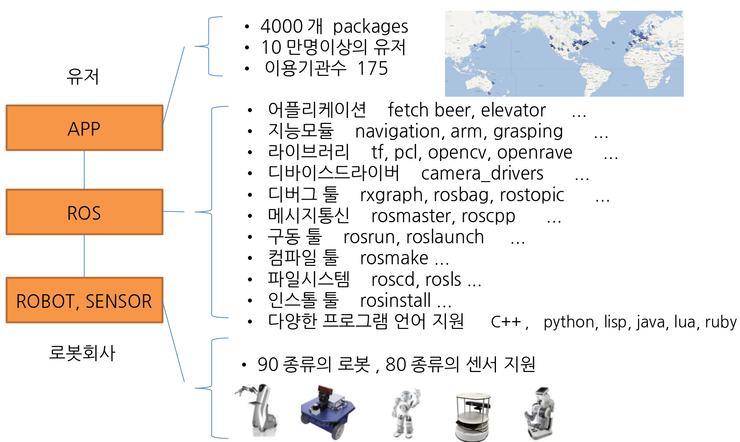
\includegraphics[width=\columnwidth]{pictures/chapter1/ecosystem.png}
\caption{ROS 에코 시스템}
\end{figure}

%-------------------------------------------------------------------------------
\section{ROS 역사}\index{ROS 역사}

%-------------------------------------------------------------------------------
\subsection{ROS 역사}\index{ROS 역사}

ROS를 본격적으로 공부하기 전에 ROS에 대해서 좀 더 알아보도록 하자. 

\begin{figure}[h]
\centering
\includegraphics[width=0.5\columnwidth]{pictures/chapter1/roslogo.png}
\caption{ROS(Robot Operating System) 로고 (http://wiki.ros.org/)}
\end{figure}

ROS는 2007년 미국의 스탠포드 대학 인공지능 연구소(AI LAB)\footnote{스탠포드대학 인공지능 연구실(AI LAB), http://ai.stanford.edu/}가 진행하던 STAIR(STanford AI Robot) 프로젝트\footnote{스탠포드대학 STAIR(STanford AI Robot) 프로젝트, http://stair.stanford.edu/}\footnote{http://stair.stanford.edu/}를 위해 Morgan Quigley \footnote{http://www.osrfoundation.org/morgan-quigley.html}이 개발한 "Switchyard" 이라는 시스템에서 시작하였다. Morgan Quigley 은 현재 ROS의 개발 및 관리를 맡고 있는 OSRF(Open Source Robotics Foundation)의 재단 설립자이며, 소프트웨어 개발 책임자이다. "Switchyard"는 그 당시 AI 연구실의 프로젝트에 사용된 인공지능 로봇의 개발을 위해 만든 프로그램이다. 

그 이외에도 2000년도 부터 개발되어, ROS 의 네트워크 프로그램에 큰 영향을 끼친 Player/Stage 프로젝트 (Player 네트워크 서버 및 2D Stage 시뮬레이터, 추후에 ROS의 3D 시뮬레이터인 Gazebo의 개발까지 영향을 미친다)\footnote{Player/Stage/Gazebo Project, http://playerstage.sourceforge.net/}의 개발자 Brian Gerkey\footnote{http://www.osrfoundation.org/brian-gerkey.html}는 OSRF의 CEO이자 재단 설립자이다. 이렇게 ROS는 2008년 윌로우게러지(Willow Garage) 회사에 의해 ROS라는 이름이 붙기전에 2000년의 "Player/Stage", 2007년의 "Switchyard" 등의 영향을 받았다.

\begin{figure}[h]
\centering
\includegraphics[width=0.5\columnwidth]{pictures/chapter1/willow_garage_logo.jpg}
\caption{윌로우게러지(Willow Garage) 로고 (http://www.willowgarage.com/)}
\end{figure}

2008년 미국의 로봇 전문 기업  윌로우게러지라는 회사가 이어받아 ROS라는 이름으로 개발하기 시작하였다. 윌로우게러지에대해 생소한 사람들도 있을지도 모르겠지만, 개인로봇(personal robotics) 및 서비스 로봇분야에서는 매우 유명하다. 그리고 우리가 알고 있는 영상처리 오픈소스인 OpenCV\footnote{OpenCV, http://opencv.org/}, 키넥트(Kinect)와 같은 3차원 디바이스에 많이 사용되고 있는 PCL(Point Cloud Library)\footnote{PCL, http://pointclouds.org/}을 개발 및 공식 지원하는 등으로도 유명하다. 

이러한 윌로우게러지는 2008년 ROS라는 이름으로 개발에 착수하였고, 2010년 1월 22일날 ROS 1.0 이라는 세상에 나왔다. 공식적으로 우리에게 알려진 버전은 ROS Box Turtle 이라는 이름으로 2010년 3월 2일 첫 릴리즈되었다. 그 뒤에도 C Turtle, Diamondback 등 버전은 우분투 및 안드로이드와 비슷하게 A B C 순으로 작명하고 있다. 최근(2014년7월)에는 ROS의 9번째 버전 ROS Indigo Igloo가 오랜 베타과정을 거치고 공개되었다. 

ROS는 BSD 라이센스를 기반으로 하고 있기에 그 누구던지 수정 편집, 재사용, 재배포가 가능하게 되었고 로봇 관련 학회를 통해 우선적으로 알려지기 시작하였다. 특히, ROSDay 및 ROSCon 이라는 이름으로 개발자 및 사용자를 대상으로 컨퍼런스 형식으로 매년 행사를 진행하고 있다. 뿐만아니라, ROS를 적용가능한 로봇 개발도 발빠르게 이루어지고 있다. 그예로 Personal Robot이라는 뜻의 PR2 footnote{PR2, http://www.willowgarage.com/pages/pr2/overview}및 터틀봇(turtlebot)\footnote{Turtlebot Official website, http://turtlebot.com/}이라는 로봇이 있으며, 이를 이용하여 많은 어플리케이션을 선보이면서 로봇 소프트웨어 플랫폼으로서 자리매김하게 되었다. 

\begin{figure}[h]
\centering
\includegraphics[width=\columnwidth]{pictures/chapter1/osrf_logo.png}
\caption{OSRF 로고 (http://osrfoundation.org/)}
\end{figure}

2007년 스탠포드 대학 인공지능 연구소에서 시작된 이 움직임은 2008년 Willow Garage \footnote{Willow Garage, http://www.willowgarage.com/}가 이어받아 그 틀을 완성하였고, 보급에 힘써왔다. 그 뒤 2013년 Willow Garage가 상업 서비스 로봇 시장으로 진입하면서 그 바톤은 오픈 소스 로봇공학 재단인 OSRF(Open Source Robotics Foundation)\footnote{OSRF, http://osrfoundation.org/}으로 이어지고 있으며, 연구소, 회사, 재단에 그치지 않고 일반 유저들도 자발적으로 ROS 개발에 참혀하고 있다. ROS 개발은 로봇공학자들의 따뜻한 관심을 받으며 앞으로도 지속될 것으로 보인다.

%-------------------------------------------------------------------------------
\subsection{ROS 의 주요 포인트}\index{ROS 의 주요 포인트}

ROS 의 릴리즈\footnote{ROS Distributions, http://wiki.ros.org/Distributions} 및 컨퍼런스

\begin{itemize}
\item 2014.09.12 ~ 13 - ROSCon2014 컨퍼런스 개최\footnote{ROSCON, http://roscon.ros.org/}
\item 2014.07.22 - Indigo Igloo 릴리즈
\item 2014.06.06 - ROS Kong 2014 개최
\item 2013.09.04 - Hydro Medusa 릴리즈
\item 2013.05.11 ~ 12 - ROSCon2013 컨퍼런스 개최
\item 2013.02 - Open Source Robotics Foundation 가 개발, 관리를 맡음
\item 2012.12.31 - Groovy Galapagos 릴리즈
\item 2012.05.19 ~ 20 - ROSCon2012 컨퍼런스 개최
\item 2012.04.23 - Fuerte Turtle 릴리즈
\item 2011.08.30 - Electric Emys 릴리즈
\item 2011.03.02 - Diamondback 릴리즈
\item 2010.08.02 - C Turtle 릴리즈
\item 2010.03.02 - Box Turtle 릴리즈
\item 2010.01.22 - ROS 1.0 개발
\item 2008 - Willow Garage 가 “ROS”라는 이름으로 개발 시작
\item 2007 - “Switchyard”, Morgan Quigley, Stanford AI LAB, 스탠포드 대학
\item 2000 - "Player/Stage Project", Brian Gerkey, Richard Vaughan, Andrew Howard, 남캘리포니아 대학
\end{itemize}


%-------------------------------------------------------------------------------
\section{ROS 버전}\index{ROS 버전}

%-------------------------------------------------------------------------------
\subsection{ROS 버전}\index{ROS 버전}

2007년 스탠포드대학 인공지능 연구소에서 "Switchyard"라는 이름으로 시작된 로봇 소프트웨어 프레임워크는 연구는, 2008년 윌로우게이지(Willow Garage)가 이어받아 "ROS(Robot Operating System)" 라는 이름으로 개발을 이어갔다. 그 뒤로 ROS 1.0을 포함하여, 7번의 버전 업데이트를 거쳐 2012.12월 ROS Groovy Galapagos 버전까지 내놓았다. 2013년에는 ROS개발이 OSRF(Open Source Robotics Foundation)으로 이양되어 현재 2014년 7월에 ROS의 9번째 버전업인 ROS Indigo Igloo 버전이 릴리즈되었다. 

\begin{figure}[h]
\centering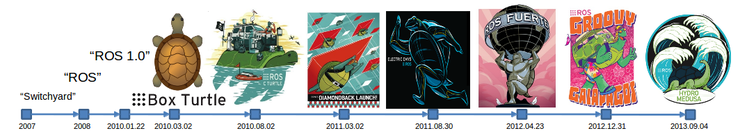
\includegraphics[width=\columnwidth]{pictures/chapter1/2013rosversion.png}
\caption{ROS 버전}
\end{figure}

%-------------------------------------------------------------------------------
\subsection{ROS 버전 규칙}\index{ROS 버전 규칙}

ROS는 2014년 8월 현재까지 ROS 1.0, Box Turtle, C Turtle, Diamondback, Electric Emys, Fuerte Turtle, Groovy Galapagos, Hydro Medusa, Indigo Igloo 의 버전을 내놓았다. 차기 버전은 Jade Turtle 로 2015년 5월에 릴리즈될 예정이다. ROS는 1.0 버전을 제외하고는 우분투와 안드로이드처럼 버전명을 A, B, C 의 알파벳 순으로 짓고 있다. 즉, 이번에 릴리즈된 Indigo Igloo 버전은 알파벳 I 버전이라는 것을 말하는 것으로 9번째 버전이다.

그 이외에도 한 가지 규칙이 더있다. 바로 각 버전마다 포스터 형식의 일러스트를 내놓으며, 거북이 아이콘을 만들어 오고 있다. 이 거북이 아이콘은 turtlesim\footnote{ROS Turtlesim, http://wiki.ros.org/turtlesim}이라는 ROS 공식 튜토리얼용 시뮬레이션에도 사용된다. ROS의 상징으로 거북이를 사용한 이유에 대해서는 특별한 설명은 없다.

\begin{figure}[h]
\centering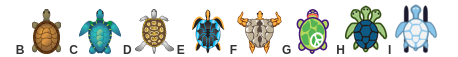
\includegraphics[width=\columnwidth]{pictures/chapter1/ros_turtle_icon.png}
\caption{caption}
\end{figure}

%-------------------------------------------------------------------------------
\subsection{ROS 버전 주기}\index{ROS 버전 주기}

지금까지 ROS는 아래와 같이 버전 업데이트\footnote{ROS 릴리즈 주기, http://wiki.ros.org/Distributions/Timeline}가 되고 있다. 초기에는 우분투의 새로운 버전의 릴리즈 주기와 동일하게 1년에 2번의 업데이트가 이루어졌다. 그러나, 2013년 빈번한 업데이트로 인하여 새로운 버전 주기를 제안하는 유저들이 생겨났다. 이에 ROS 개발 및 관리를 맡은 OSRF는 유저들의 의견을 수렴하여 2013년 Hydro Medusa 버전 부터는 1년에 1번 정식 버전을 릴리즈하며 그 시기는 우분투의 새로운 버전 출시인 4월에 하기로 결정이 내려졌다. 올해는 새로운 버전 주기를 새로 세우면서 버전 주기가 불안정했지만 내년 2014년 부터는 매년 4월에 새로운 버전의 정식 릴리즈가 이루어질 예정이다.

\begin{figure}[h]
\centering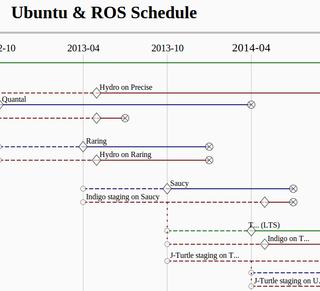
\includegraphics[width=0.5\columnwidth]{pictures/chapter1/ros_timeline.png}
\caption{caption}
\end{figure}

또한, ROS는 공식 지원 운영체제로 우분투(Ubuntu) LTS를 지원한다. 지원하는 우분투 버전은 2년에 한 번씩 릴리즈 되는 우분투 LTS(Long Term Support, 5년간 지원하는 버전) 주기 에 맞추기로 하였다. 즉, 2014년의 우분투 14.04 LTS 를 지원하는 ROS 버전은 2014년의 ROS I 와 2015년의 J 버전 이렇게 두 개의 버전이 지원될 예정이다.

\begin{itemize}
\item 2015.05.01 - Jade Turtle (예정)
\item 2014.07.22 - Indigo Igloo\footnote{ROS Hydro Medusa, http://wiki.ros.org/indigo} (현재)
\item 2013.09.04 - Hydro Medusa\footnote{ROS Hydro Medusa, http://wiki.ros.org/hydro}
\item 2012.12.31 - Groovy Galapagos\footnote{ROS Groovy Galapagos, http://wiki.ros.org/groovy}
\item 2012.04.23 - Fuerte Turtle\footnote{ROS Fuerte Turtle, http://wiki.ros.org/fuerte}
\item 2011.08.30 - Electric Emys\footnote{ROS Electric Emys, http://wiki.ros.org/electric}
\item 2011.03.02 - Diamondback\footnote{ROS Diamondback, http://wiki.ros.org/diamondback}
\item 2010.08.02 - C Turtle\footnote{ROS C Turtle, http://wiki.ros.org/cturtle}
\item 2010.03.02 - Box Turtle\footnote{ROS Box Turtle, http://wiki.ros.org/boxturtle}
\item 2010.01.22 - ROS 1.0
\end{itemize}

%-------------------------------------------------------------------------------
\subsection{ROS 최신 버전}\index{ROS 최신 버전}

\begin{figure}[h]
\centering
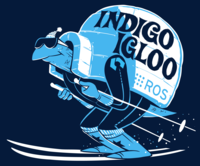
\includegraphics[width=0.4\columnwidth]{pictures/chapter1/indigo_igloo.png}

\includegraphics[width=0.3\columnwidth]{pictures/chapter1/indigo_igloo_icon.png}
\caption{caption}
\end{figure}

2014년 07월 22일, 정식 릴리즈된 ROS Indigo Igloo\footnote{ROS Indigo Igloo, http://wiki.ros.org/indigo/}가 현재 ROS의 최신 버전이다. 포스터는 거북이가 이글루(Igloo)을 등에 엎고 있는 모습이고, 아이콘에는 스키는 타는 재미난 모습을 담고 있다.

이번 버전은 무엇보다 더욱 catkin 빌드 시스템에 중점을 두어 모든 패키지가 catkin화 되었다는 점이다. 그 이외에는 이번 버전 부터는 Python3.3 을 사용하였다는 점, 내부적으로는 아직 Python2가 주이기는 하지만 Python3도 사용 가능하는 것을 의미한다. 그리고, OpenCV를 우분투 표준의 것을 이용한다는 점, cmake modules 라는 패키지가 있는데 이는 공식 서포트하지 않는 패키지들을 모아 두었다는 점, boost의 signal함수의 사용을 모두 signal2로 변경하여 최신의 버전을 유지하였다는 점으로 전체적으로 마이너 업그레이드와 유지보수으 성격이 강하다.

ROS Indigo Igloo에 대한 더 자세한 정보는 아래의 링크를 참조하기 바란다.

%-------------------------------------------------------------------------------
\subsection{ROS 버전 선택}\index{ROS 버전 선택}

ROS는 메타운영체제이기때문에 기본적으로 사용하는 OS를 선택해야한다. ROS는 Ubuntu, OS X, Fedora, Gentoo, OpenSUSE, Debian, Arch Linux, Windows 등을 지원하고 있지만, ROS 유저들이 제일 많이 사용하고 있는 OS는 우분투라고 할 수 있다. 개발팀에서도 우분투 LTS 버전\footnote{우분투 릴리즈 주기, https://wiki.ubuntu.com/Releases}에 맞추어 테스트를 진행하고 릴리즈하고 있다. 이러한 이유로 필자는 ROS LTS 버전에 맞는 ROS 버전을 선택하라고 말하고 싶다. 

각각의 ROS 버전에 대한 우부투 포팅에 대한 정보는 http://www.ros.org/debbuild/ 에 접속하여 사용하고자하는 ROS 버전의 이름의 html 을 보도록 하자. 이 파일에는 현재 선택한 ROS 버전이 1행의 우분투 버전별로 기존 패키지(소스)가 이전작업이 완료되었는지 진행중인지 볼 수 있다. 여기서 우분투 버전이 생소한데, 아래의 우분투 버전을 보면 11.04가 N으로 표기되어 있으며, 그 뒤로 O, P, Q, R, S 로 진행되고 있다. 이를 비교하여 안정화된 버전을 찾아야한다. ROS의 최신 버전의 경우에는 많은 패키지가 작업중으로 뜨는데 중요한 패키지가 아니고서는 문제 없으니 바로 최신 버전을 사용해도 좋고, 자신이 사용하던 패키지가 새로운 ROS 버전에 적용이 안되었다면 좀 더 기다릴 필요가 있다고 할 수 있다. 

\begin{itemize}
\item Ubuntu 14.04 Trusty Tahr (LTS)
\item Ubuntu 13.10 Saucy Salamander
\item Ubuntu 13.04 Raring Ringtail 
\item Ubuntu 12.10 Quantal Quetzal 
\item Ubuntu 12.04 Precise Pangolin (LTS)
\item Ubuntu 11.10 Oneiric Ocelot
\item Ubuntu 11.04 Natty Narwhal
\item Ubuntu 10.10 Maverick Meerkat
\item Ubuntu 10.04 Lucid Lynx (LTS)
\end{itemize}

2014년 8월 11일 현재, 필자는 아래와 같은 조합을 추천하고자 한다.

\begin{itemize}
\item Ubuntu 14.04 Trusty Tahr (LTS)
\item ROS Indigo Igloo
\end{itemize}

% \begin{enumerate}
% \item The first item
% \item The second item
% \item The third item
% \end{enumerate}

% \subsection{Bullet Points}\index{Lists!Bullet Points}

% \begin{itemize}
% \item The first item
% \item The second item
% \item The third item
% \end{itemize}

% \subsection{Descriptions and Definitions}\index{Lists!Descriptions and Definitions}

% \begin{description}
% \item[Name] Description
% \item[Word] Definition
% \item[Comment] Elaboration
% \end{description}